%! Author = Kyle Baldes
%! Date = 10/1/23

% Preamble
\documentclass[11pt]{article}

% Packages
\usepackage{amsmath}
\usepackage{graphicx}
\usepackage{tikz}
\usetikzlibrary{positioning, shapes.geometric}
\usepackage{adjustbox}

\begin{document}

\section*{Entity Relationship Diagram}
%\begin{adjustbox}{left}
    \begin{figure}[h]
        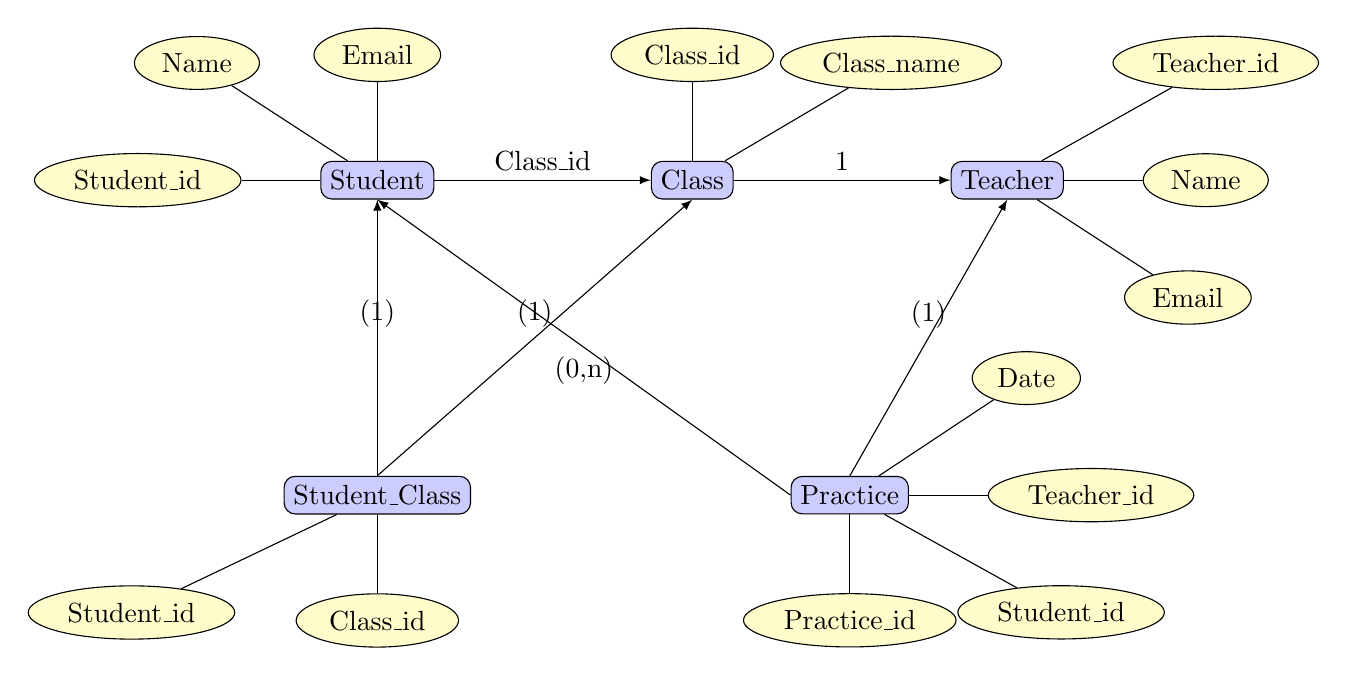
\begin{tikzpicture}[entity/.style={rectangle, draw=black, fill=blue!20, rounded corners},
                                attribute/.style={shape=ellipse, draw=black, fill=yellow!20},
                                link/.style={->,>=latex}]
            % Student Entity
            \node[entity] (student) at (0,0) {Student};
            \node[attribute] (studentid) [left=of student] {Student\_id} edge (student);
            \node[attribute] (sname) [above left=of student] {Name} edge (student);
            \node[attribute] (semail) [above=of student] {Email} edge (student);

            % Class Entity
            \node[entity] (class) at (4,0) {Class};
            \node[attribute] (classid) [above =of class] {Class\_id} edge (class);
            \node[attribute] (classname) [above right=of class] {Class\_name} edge (class);

            % Teacher Entity
            \node[entity] (teacher) at (8,0) {Teacher};
            \node[attribute] (teacherid) [above right=of teacher] {Teacher\_id} edge (teacher);
            \node[attribute] (tname) [right =of teacher] {Name} edge (teacher);
            \node[attribute] (temail) [below right=of teacher] {Email} edge (teacher);

            % Student_Class Entity
            \node[entity] (studentclass) at (0,-4) {Student\_Class};
            \node[attribute] (scstudentid) [below left=of studentclass] {Student\_id} edge (studentclass);
            \node[attribute] (scclassid) [below=of studentclass] {Class\_id} edge (studentclass);

            % Practice Entity
            \node[entity] (practice) at (6,-4) {Practice};
            \node[attribute] (practiceid) [below=of practice] {Practice\_id} edge (practice);
            \node[attribute] (pstudentid) [below right=of practice] {Student\_id} edge (practice);
            \node[attribute] (pteacherid) [right=of practice] {Teacher\_id} edge (practice);
            \node[attribute] (pdate) [above right=of practice] {Date} edge (practice);

            % Relationships
            \draw[link] (student) -- node[midway,above]{Class\_id} (class);
            \draw[link] (class) -- node[midway,above]{1} (teacher);
            \draw[link] (studentclass.north) -- node[midway,above]{(1)} (student.south);
            \draw[link] (studentclass.north) -- node[midway,above]{(1)} (class.south);
            \draw[link] (practice.west) -- node[midway,below]{(0,n)} (student.south);
            \draw[link] (practice.north) -- node[midway,above]{(1)} (teacher.south);
        \end{tikzpicture}\label{fig:figure}
    \end{figure}
%\end{adjustbox}

\end{document}